\section{二氧化碳}\label{sec:3-4}

碳元素除组成多种单质外,还组成各种化合物。这里只学习几种简单的碳的化合物。
首先学习碳的氧化物。在碳的氧化物里,最常见的是二氧化碳。

\subsection{二氧化碳的性质}

\begin{shiyan}
    在天平的一个托盘上,放置一个 250 毫升的烧杯,用砝码使天平两边达到平衡。
    取一瓶二氧化碳气体,先观察二氧化碳的颜色,然后把它慢慢地倾注到托上的烧杯里(图 \ref{fig:3-5}),
    仔细观察天平两边是否还保持平衡,为什么?
\end{shiyan}

\begin{figure}[htbp]
    \centering
    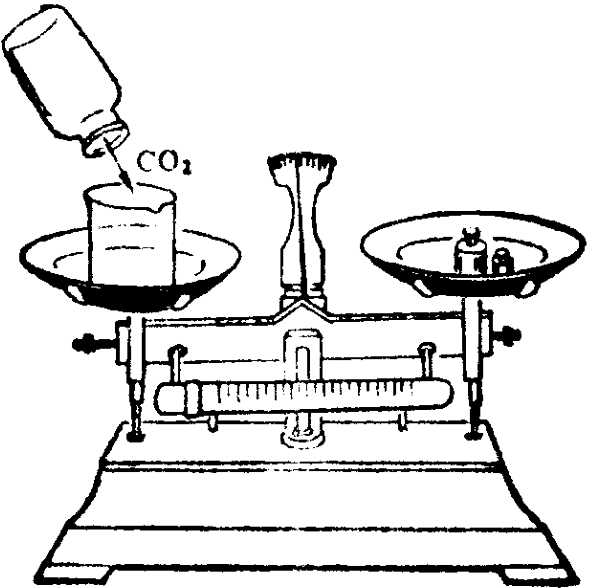
\includegraphics[width=8cm]{../pic/czhx1-ch3-5}
    \caption{向烧杯里倾倒二氧化碳}\label{fig:3-5}
\end{figure}

二氧化碳是一种比空气重、没有颜色的气体。可以象倾倒液体那样,把二氧化碳从一个容器倒到另一个容器里。
在标准状况下,二氧化碳的密度是 $1.977 \; \kms$。
在通常状况下,1 体积的水约能溶解 1 体积的二氧化碳,增加压强会溶解得更多些。
汽水是将二氧化碳加压溶解在水里制成的。
在加压和冷却的情况下,二氧化碳变成无色的液体,温度再降低,还能够变成雪状的固体。
经过压缩的二氧化碳固体叫做 “干冰”。
在 1 标准大气压下,“干冰” 在 $-78.5$ ℃ 时直接变成二氧化碳气体。

\begin{shiyan}
    点着两支短蜡烛,分别放在一个梯形的小白铁皮架的两个阶梯上,把白铁皮架放在烧杯里。
    按图 \ref{fig:3-6}所示,向烧杯里倾倒二氧化碳。注意观察两支蜡烛先后分别发生的现象。
\end{shiyan}

\begin{figure}[htbp]
    \centering
    \begin{minipage}[b]{7cm}
        \centering
        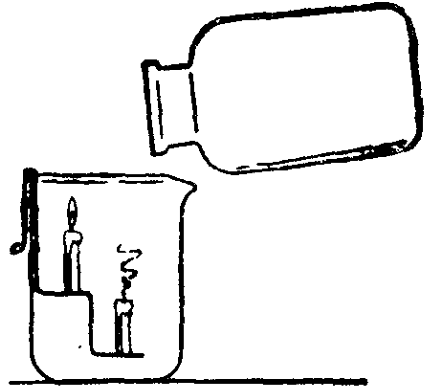
\includegraphics[width=4cm]{../pic/czhx1-ch3-6}
        \caption{二氧化碳熄灭蜡烛火焰}\label{fig:3-6}
    \end{minipage}
    \qquad
    \begin{minipage}[b]{7cm}
        \centering
        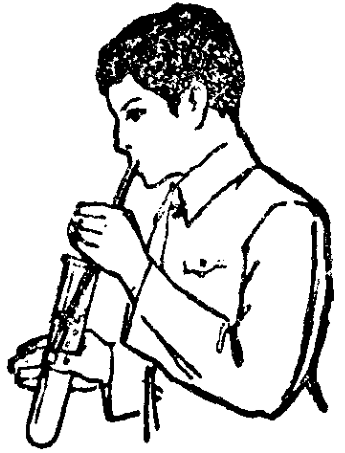
\includegraphics[width=4cm]{../pic/czhx1-ch3-7}
        \caption{向澄清石灰水里吹二氧化碳}\label{fig:3-7}
    \end{minipage}
\end{figure}


在一般情况下,二氧化碳既不能燃烧,也不能支持燃烧。二氧化碳不能供给呼吸。

\begin{yuedu}
    二氧化碳不能供给呼吸,在二氧化碳过多而氧气不足的地方,人们会感到窒息。
    通常空气里含二氧化碳 $0.03\%$。
    空气里二氧化碳含量达 $1\%$ 的时候,对人就有害处,
    达 $4 \text{—} 5\%$ 的时候,便会使人到气喘、头痛、眩晕,
    达 $10\%$ 的时候, 能使人不省人事, 呼吸逐渐停止,以致死亡。
\end{yuedu}

干涸的深井、深洞和久未开启的甘薯窖或白菜窖的底部,二氧化碳的浓度较大,
在进入这些地方前,须先用灯火试验,如灯火熄灭或燃烧得不旺,就不要进去。

\begin{shiyan}
    向紫色石蕊\footnote{石蕊是一种色素,遇酸变成红色。}试液里通入二氧化碳,观察石蕊试液颜色的变化。
\end{shiyan}

二氧化碳溶解在水里,生成碳酸(\ce{H2CO3})。
\begin{fangchengshi}
    \ce{ CO2 + H2O = H2CO3 }
\end{fangchengshi}

碳酸能使石蕊试液变成红色,只是颜色浅些。
碳酸分子里的 \ce{CO3} 部分是一个原子团,叫做碳酸根。

\begin{shiyan}
    通过一根约 15 厘米长的玻璃管,向澄清的石灰水里吹气(图\ref{fig:3-7})。观察石灰水发生的变化。
\end{shiyan}


人们向澄清的石灰水〔\ce{Ca(OH)2} 溶液〕里吹入二氧化碳时,就会发生反应,
使石灰水变浑浊,这是由于生成白色的碳酸钙沉淀的缘故。这个反应可以用化学方程式表示如下:
\begin{fangchengshi}
    \ce{ CO2 + Ca(OH)2 = \underset{\text{碳酸钙}}{\ce{CaCO3}} v + H2O }
\end{fangchengshi}

常用这个反应来鉴定二氧化碳。


\subsection{二氧化碳的制法}

\begin{wrapfigure}[12]{r}{5cm}
    \centering
    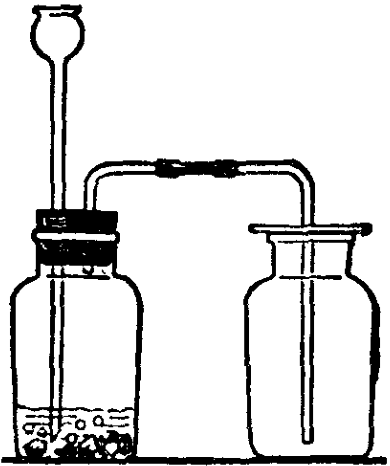
\includegraphics[width=4cm]{../pic/czhx1-ch3-8}
    \caption{制取二氧化碳的装置}\label{fig:3-8}
\end{wrapfigure}

在实验室里,二氧化碳常用稀盐酸跟大理石或石灰石(主要成分都是 \ce{CaCO3})起反应而制得。

\begin{shiyan}
    图 \ref{fig:3-8} 是制取二氧化碳的装置。
    在左边的广口瓶里放些大理石的小块,
    从长颈漏斗注入稀盐酸(为了防止气体从长颈漏斗逸出,需将漏斗下端插入液面以下)。
    注意观察广口瓶里生的变化。
    怎样用集气瓶收二氧化碳?怎样证明集气瓶里已充满了二氧化碳?
\end{shiyan}


由于二氧化碳能溶于水,比空气重,所以不能用排水法收集,但可用向上排空气法收集在集气瓶里。
用燃着的火柴放在集气瓶口试验,如果火焰熄灭,证明瓶里已充满了二氧化碳。

这个反应的化学方程式可表示如下:
\begin{fangchengshi}
    \ce{ CaCO3 + 2HCl = $\underset{\text{氯化钙}}{\ce{CaCl2}}$ + H2CO3 }
\end{fangchengshi}

碳酸钙跟盐酸起反应,先生成氯化钙和碳酸,而碳酸是一种很不稳定的物质,容易分解成二化碳和水。
\begin{fangchengshi}
    \ce{ H2CO3 = H2O + CO2 ^ }
\end{fangchengshi}

碳酸钙跟盐酸起反应的总的化学方程式是:
\begin{fangchengshi}
    \ce{ CaCO3 + 2HCl = CaCl2 + H2O + CO2 ^ }
\end{fangchengshi}

工业上在高温下煅烧石灰石来制取生石灰(\ce{CaO}), 同时生成的二氧化碳是副产品。
\begin{fangchengshi}
    \ce{ CaCO3 $\xlongequal{\text{高温}}$ CaO + CO2 ^ }
\end{fangchengshi}


\subsection{二氧化碳的用途}

二氧化碳不能支持燃烧,又比空气重,如果让二氧化碳覆盖在燃着的物体上,就能使物体跟空气隔绝而停止燃烧。
因此二氧化碳可以用来灭火。通常的灭火器就是利用化学反应产生的二氧化碳来灭火的一种设备,
灭火器里的二氧化碳是由硫酸跟碳酸钠(\ce{Na2CO3}) 起反应来制取的。
\begin{fangchengshi}
    \ce{ Na2CO3 + H2SO4 = Na2SO4 + H2O + CO2 ^ }
\end{fangchengshi}

\begin{shiyan}
    在吸滤瓶里注入碳酸钠的浓溶液,把盛有浓盐酸\footnote{这里用浓盐酸代替硫酸。}的小试管系住,
    小心地放进吸滤瓶(注意:不要使浓盐酸流出),把塞子塞紧(图 \ref{fig:3-9} I)。
    然后把吸滤瓶倒转过来(图 \ref{fig:3-9} II),使两种溶液混和,注意观察吸滤瓶的侧管
    {\large \heiti(要注意安全,实验者切勿让侧管对着别人或自己)}
    有什么现象发生?为什么?
\end{shiyan}

\begin{figure}[htbp]
    \centering
    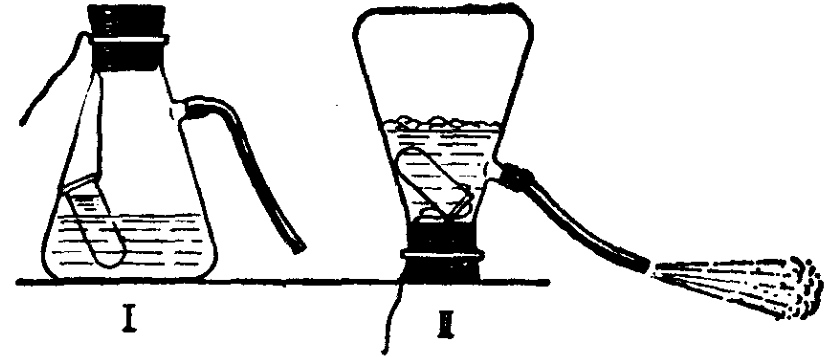
\includegraphics[width=8cm]{../pic/czhx1-ch3-9}
    \caption{灭火器原理}\label{fig:3-9}
\end{figure}


通常使用的灭火器有泡沫灭火器、干粉灭火器和液态二氧化碳灭火器等。

\begin{yuedu}
    泡沫灭火器里除装有用于产生二氧化碳的原料外,还有能产生泡沫的
    物质\footnote{在常用的泡沫灭火器里,用硫酸铝〔\ce{Al2(SO4)3}〕来代替硫酸,
        并用碳酸氢钠(\ce{NaHCO3})来代替碳酸钠。
        为了发生泡沫,常放人用甘草或皂角等作原料制取的液体。
    }。
    泡沫灭火器的原理和上面介绍的灭火器原理是一致的。

    干粉灭火器是用压缩的二氧化碳吹干粉\footnote{干粉主要含有碳酸氢钠等物质。}作灭火剂的,
    干粉具有流动性好、喷射率高、不腐蚀容器和不易变质等优良性能。

    在加压的情况下,把液态二氧化碳装入小钢瓶里,可以制成液态二氧化碳灭火器。
    这种灭火器可以用在不适于用水扑灭的油类或电器着火上。(为什么不能用水扑灭这类火呢?)
    当打开阀门的时候,喷出的二氧化碳生成一层气体覆盖层,使火焰立即熄灭,而物体不会损坏。
\end{yuedu}

二氧化碳也是一种工业原料,可以用在制纯碱、尿素、糖和汽水等工业上。

“干冰” 可用作致冷剂,用来保藏很容易腐败的食品。
因为 “干冰” 蒸发以后,没有液体留下,不会使食品潮湿。
用飞机从高空撒布 “干冰”, 能够使空气里的水蒸气冷凝,变成水滴下降。
这是人工降雨的一种方法。

植物进行光合作用,需要二氧化碳,生成糖和淀粉。
在温室里施用二氧化碳作肥料,可以提高农作物的产量。


\liti[0] 有半瓶稀盐酸,内含氯化氢 60 克,使这些氯化氢跟 75 克碳酸钙起反应,
可制得二氧化碳多少克?反应后,两种反应物中哪一种过剩?剩余多少克?

\jie 首先通过计算判断哪一种反应物过剩。

设 $x$ 为跟 75 克碳酸钙起反应所需的氯化氢的克数,并设 $y$ 为生成的二氧化碳的克数。
\begin{fangchengshi}
    \dengshi{0}{-1}{
        2(35.5 + 1) \\
        =73 \\
        x \ke
    }
    \dengshi{2.5}{-1}{
        40 + 12 + 16 \times 3  \\
        = 100  \\
        75 \ke
    }
    \dengshi{6.5}{-1}{
        12 + 16 \times 2\\
        = 44  \\
        y \ke
    }
    \ce{ 2HCl + CaCO3 = CaCl2 + H2O + CO2 ^ } \\[4em]
\end{fangchengshi}

先求所需氯化氢克数
\begin{align*}
    & 73:100 = x:75 \\
    & x = \dfrac{73 \times 75}{100} = \dfrac{219}{4} = 54.7 \; (\ke)
\end{align*}

反应所需氯化氢比反应物中的氯化氢少 $60 - 54.7 = 5.3 \;(\ke)$, 说明原料中氯化氢过剩 5.3 克。

然后根据没有过剩的即反应完全的那种反应物碳酸钙的量,计算制得的二氧化碳的量。
\begin{align*}
    & 100:44 = 75:y \\
    & y = \dfrac{44 \times 75}{100} = 33 \; (\ke)
\end{align*}

答:可制得二氧化碳 33 克,在两种反应物中氯化氢过剩, 剩余 5.3 克。



\begin{xiti}

\xiaoti{选择正确的答案填写在括号里。}
\begin{xiaoxiaotis}

    \xxt{二氧化碳是 \ewkh 。\\
        \tc{1} 无色的气体, \tc{2}一种有刺鼻气味的气体, \tc{3} 一种有毒的气体, \tc{4} 一种黄烟。
    }


    \xxt{二氧化碳能够灭火是因为 \ewkh 。\\
        \tc{1} 它是气体, \tc{2} 它在高压低温下能变成“干冰”,\\
        \tc{3} 它不能燃烧,也不支持燃烧, \tc{4}它溶于水。
    }

\end{xiaoxiaotis}


\xiaoti{为了使石灰浆〔\ce{Ca(OH)2}〕抹的墙壁快点干燥,常常在室内生个炭火盆。
    为什么在放炭火盆的开始,墙壁反而更潮湿?写出反应的化学方程式。
}


\xiaoti{下述反应都能生成二氧化碳气体吗?如果能,写出反应的相应化学方程式。}
\begin{xiaoxiaotis}

    \xxt{碳酸钾(\ce{K2CO3})跟稀硫酸起反应,}

    \xxt{木炭在空气里燃烧,}

    \xxt{煅烧石灰石,}

    \xxt{大理石跟盐酸起反应。}

\end{xiaoxiaotis}


\xiaoti{把氧化铜跟木炭粉各 1.59 克混和,放在大试管里加热。
    反应完毕后,生成铜多少克?如果反应物中有过剩的,指出是哪一种,并计算剩余多少?
}

\end{xiti}

